\documentclass[a4paper,12pt]{article}

\usepackage[utf8]{inputenc}
\usepackage{graphicx}
\usepackage{amsmath}
\usepackage{amssymb}
\usepackage{hyperref}
\usepackage{geometry}
\usepackage{tikz}
\usepackage{wrapfig}
\usetikzlibrary{shapes, positioning}

%% Plan aesthetics
\usepackage{listings}
\usepackage{xcolor}

\definecolor{codegreen}{rgb}{0,0.6,0}
\definecolor{codegray}{rgb}{0.5,0.5,0.5}
\definecolor{codepurple}{rgb}{0.58,0,0.82}
\definecolor{backcolour}{rgb}{0.95,0.95,0.92}

\lstdefinestyle{mystyle}{
    backgroundcolor=\color{backcolour},   
    commentstyle=\color{codegreen},
    keywordstyle=\color{magenta},
    numberstyle=\tiny\color{codegray},
    stringstyle=\color{codepurple},
    basicstyle=\ttfamily\footnotesize,
    breakatwhitespace=false,         
    breaklines=true,                 
    captionpos=b,                    
    keepspaces=true,                 
    numbers=left,                    
    numbersep=5pt,                  
    showspaces=false,                
    showstringspaces=false,
    showtabs=false,                  
    tabsize=2
}
\lstset{style=mystyle}
%%%%%%%%%%%%%%%%%%%%%%%%%%%%%%%%%%%%%%5


\geometry{margin=1in}

\title{Robot Chef Task Report}
\author{Mauro Vázquez Chas \\
Ismael Ruiz Garcia \\
Mácsai Dániel
}
\date{\today}

\begin{document}

\maketitle

\begin{abstract}
    This report describes the development and implementation of the Robot Chef task. The objective of this project is to automate meal preparation in a structured kitchen environment using a planning algorithm implemented in PDDL. For this project, we utilized the Best First Width Search (BFWS) planner to enable the robot to handle various recipes—such as tortilla, sushi, and paella—each requiring specific preparation steps across different kitchen zones. The task begins with a scenario where tools are misplaced and dirty, requiring the robot to clean, relocate, and organize the tools before proceeding with tasks like cutting, cooking, and mixing to prepare the ingredients.
\end{abstract}

\newpage
\tableofcontents
\newpage

\section{Introduction}
\label{sec:introduction}
Provide an introduction to the project, including background information and objectives.
\begin{wrapfigure}{r}{0.5\textwidth}
    \centering
    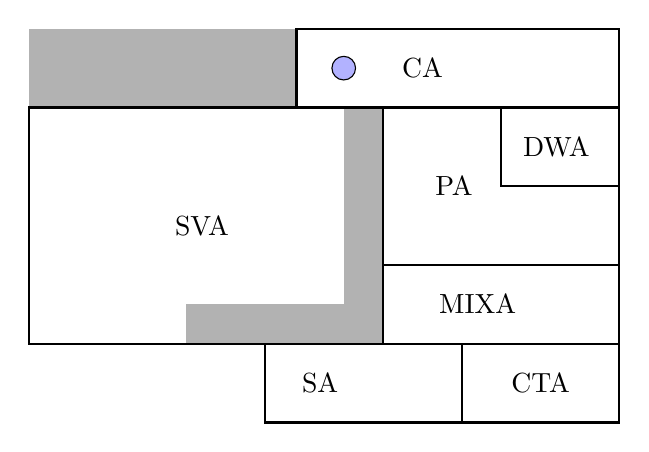
\begin{tikzpicture}
        % Define some colors for convenience
        \definecolor{wallcolor}{rgb}{0.7,0.7,0.7} % wall color
        \definecolor{chaircolor}{rgb}{0.7,0.9,1.0} % chair color
        \definecolor{redcolor}{rgb}{1.0,0.8,0.8} % red area color
        
        % Draw walls
        \fill[wallcolor] (0,4) rectangle (3.4,3); % top horizontal wall
        \fill[wallcolor] (4,0) rectangle (4.5,3); % vertical wall on the right of SVA
        \fill[wallcolor] (2,0.5) rectangle (4.5,0); % bottom horizontal wall
        
        % Room divisions
        \draw[thick] (0,0) rectangle (4.5,3); % outer rectangle (overall structure)
        \draw[thick] (3,-1) rectangle (5.5,0); % SA 
        \draw[thick] (5.5,-1) rectangle (7.5,0); % CTA
        \draw[thick] (4.5,1) rectangle (7.5,0); % MIXA
        \draw[thick] (4.5,3) rectangle (7.5,1); % PA
        \draw[thick] (6,3) rectangle (7.5,2); % DWA
        \draw[thick] (3.4,3) rectangle (7.5,4); % CA
        
    
        % Labels
        \node at (2.2,1.5) {SVA}; % SVA label
        \node at (3.7,-0.5) {SA}; % SA label
        \node at (5.4,2) {PA}; % PA label
        \node at (6.7,2.5) {DWA}; % DWA label
        \node at (6.5,-0.5) {CTA}; % CTA label
        \node at (5.7,0.5) {MIXA}; % MIXA label
        \node at (5,3.5) {CA}; % CA label
        
        
        % Person icon
        \node[draw, circle, fill=blue!30, inner sep=0pt, minimum size=0.3cm] at (4,3.5) {}; % Person circle icon
    \end{tikzpicture}
    \caption{Kitchen layout}
    \label{fig:kitchen_layout}
\end{wrapfigure}

This assignment involves designing a plan for a robot chef operating within the structured environment of a Japanese restaurant kitchen in Barcelona to autonomously handle meal preparation tasks. The robot’s objective is to receive digital orders, gather required ingredients, perform necessary preparation and cooking steps, and plate finished dishes for serving. Operating within a divided kitchen layout, the robot must navigate across specific areas for storage, preparation, cooking, serving, and dishwashing, while adhering to operational constraints such as limited carrying capacity and the need for tool sanitation after each use.

The planning solution is implemented using the Planning Domain Definition Language (PDDL), which defines the necessary actions, predicates, and conditions to enable the robot to effectively fulfill its tasks. This report provides a comprehensive analysis of the problem, including the structure of the PDDL model, testing cases across different scenarios, and results demonstrating the robot’s adaptability to diverse dish requirements, resource management, and task optimization. The following sections detail the problem setup, solution framework, and evaluation of scenario-based testing to assess the robot’s performance, efficiency, and flexibility.

\section{Methodology and implementation details}
\label{sec:methodology}
We now define the predicates and actions that we are using in the PDDL implementation. The predicates define the state of the world (in this case, the kitchen and its elements), such as valid rooms and their adjacencies, the location of tools, and the condition of ingredients. Actions describe the possible operations the robot can perform, including moving around the kitchen, picking up items (tools, ingredients and dishes), and using them to assemble the required dishes.

\subsection{Predicates}
\begin{itemize}
    \item \texttt{(at ?x - portable ?y - room)}: A \textit{portable} object \textbf{?x} is located in a specific \textit{room} \textbf{?y}.
    \item \texttt{(clean ?tool - tool)}: The \textit{tool} \textbf{?tool} is clean.
    \item \texttt{(holding ?x - item)}: The robot is holding the \textit{item} \textbf{?x}.
    \item \texttt{(not-holding)}: The robot is not holding anything.
    \item \texttt{(adjacent ?room1 - room ?room2 - room)}: \textit{Room} \textbf{?room1} is adjacent to \textit{room} \textbf{?room2}.
    \item \texttt{(dish-prepared ?dish - dish)}: The \textit{dish} \textbf{?dish} has been prepared.
    \item \texttt{(dish-served ?dish - dish)}: The \textit{dish} \textbf{?dish} has been served.
    \item \texttt{(prioritize ?dish1 ?dish2)}: \textit{Dish} \textbf{?dish1} has higher priority than \textit{dish} \textbf{?dish2}.
    \item \texttt{(is-storage ?room - room)}: \textit{Room} \textbf{?room} functions as a storage area.
    \item \texttt{(is-cooking ?room - room)}: \textit{Room} \textbf{?room} is designated for cooking activities.
    \item \texttt{(is-serving ?room - room)}: \textit{Room} \textbf{?room} is designated for serving activities.
    \item \texttt{(is-preparation ?room - room)}: \textit{Room} \textbf{?room} is designated for preparation activities.
    \item \texttt{(is-dishwashing ?room - room)}: \textit{Room} \textbf{?room} is designated for dishwashing activities.
    \item \texttt{(tool-use-room ?tool - tool ?room - room)}: The \textit{tool} \textbf{?tool} is used in \textit{room} \textbf{?room}.
    \item \texttt{(ingredient-prep-room ?ingredient - ingredient ?room - room)}: The \textit{ingredient} \textbf{?ingredient} is prepared in \textit{room} \textbf{?room}.
    \item \texttt{(ingredient-stored ?ingredient - ingredient)}: The \textit{ingredient} \textbf{?ingredient} is stored.
    \item \texttt{(ingredient-available ?ingredient - ingredient)}: The \textit{ingredient} \textbf{?ingredient} is available for use.
    \item \texttt{(ingredient-prepared ?ingredient - ingredient)}: The \textit{ingredient} \textbf{?ingredient} has been prepared.
    \item \texttt{(ingredient-cooked ?ingredient - ingredient)}: The \textit{ingredient} \textbf{?ingredient} has been cooked.
    \item \texttt{(ingredient-in-dish ?ingredient - ingredient ?dish - dish)}: The \textit{ingredient} \textbf{?ingredient} is included in the \textit{dish} \textbf{?dish}.
    \item \texttt{(require-prepared ?dish - dish ?ingredient - ingredient)}: The \textit{dish} \textbf{?dish} requires the \textit{ingredient} \textbf{?ingredient} to be prepared.
    \item \texttt{(require-cooked ?dish - dish ?ingredient - ingredient)}: The \textit{dish} \textbf{?dish} requires the \textit{ingredient} \textbf{?ingredient} to be cooked.
\end{itemize}

\subsection{Actions}

\begin{itemize}
    \item \texttt{move}:  Robot transitions from one room to another. It requires three parameters: the robot itself, the room it is moving from, and the room it is moving to. The precondition for this action is that the robot must currently be in the room it is moving from, and the destination room must be adjacent to the current room. Upon successful execution of the action, the robot will be located in the new room, and it will no longer be in the original room.

    \item \texttt{pick-up}: The robot picks up an item in the same room. The action is defined with the following parameters: a robot, an item, and a room. The precondition for this action is that both the robot and the item must be in the same room, and the robot must not be holding anything.

    \item \texttt{pick-up-ingredient}: The robot retrieves an ingredient from storage. Parameters include a robot, an ingredient, a dish, and a room. Preconditions require the robot and ingredient to be in the storage room, the ingredient to be stored, the robot not holding anything, and the ingredient to be part of the dish. The effect is that the robot holds the ingredient, the ingredient becomes available, and it is no longer stored.

    \item \texttt{drop-tool}: The robot drops a tool in a designated room. Parameters include a robot, a tool, and a room. Preconditions require the robot to be in the room, holding the tool, and the tool to be used in that room. The effect is that the robot is no longer holding the tool, and the tool is located in the room.
    
    \item \texttt{drop-ingredient-at-prep}: The robot drops an ingredient in a preparation room. Parameters include a robot, an ingredient, and a room. Preconditions require the robot to be in the room, holding the ingredient, and the room to be either designated for ingredient preparation or a general preparation room. The effect is that the robot is no longer holding the ingredient, the robot is not holding anything, and the ingredient is located in the room.
    
    \item \texttt{prepare-ingredient}: The robot prepares an ingredient using a tool in a designated room. Parameters include a robot, an ingredient, a tool, and a room. Preconditions require the robot and ingredient to be in the preparation room, the robot to hold the tool, the tool to be used in that room, and the tool to be clean. The effect is that the ingredient becomes prepared, and the tool is no longer clean.

    \item \texttt{cook-ingredient}: The robot cooks a prepared ingredient in the cooking room. Parameters include a robot, an ingredient, and a room. Preconditions require the room to be designated for cooking, the robot to be in the cooking room, the ingredient to be prepared, and the robot to be holding the ingredient. The effect is that the ingredient becomes cooked.

    \item \texttt{assemble-dish}: The robot assembles a dish in the preparation room. Parameters include a robot, a dish, and a room. Preconditions require the robot to be in the preparation room. The \texttt{forall} function is used to ensure that for every ingredient in the dish, if the dish requires the ingredient to be prepared, then the ingredient must be prepared and located in the room. Similarly, if the dish requires the ingredient to be cooked, then the ingredient must be cooked and located in the room. The effect is that the dish becomes prepared and is located in the room. The \texttt{forall} function is also used in the effect to ensure that for every ingredient in the dish, the ingredient is no longer available, prepared or cooked, as well as not located in the room.

     The \textit{forall} function in PDDL is used to specify conditions that must hold for all objects of a certain type. In the context of the \texttt{assemble-dish} action, it ensures that the preconditions and effects apply to all ingredients that are part of the dish. This allows the robot to verify and update the state of each ingredient in relation to the dish being assembled, ensuring that all necessary conditions are met for the dish to be considered prepared.

    \item \texttt{plate-dish}: The robot plates a prepared dish in the serving room. Parameters include a robot, a room, and a dish. Preconditions require the room to be designated for serving, the robot to be in the serving room, the robot to hold the dish, and the dish to be prepared. The effect is that the dish becomes served, and the robot is no longer holding the dish.
    
    
    \item \texttt{clean-tool}: The robot cleans a tool in the dishwashing room. Parameters include a robot, a tool, and a room. Preconditions require the robot to be in the dishwashing room, holding the tool, and the tool not being clean. The effect is that the tool becomes clean.

\end{itemize}

\section{Results}
\subsection{Problem 1}
\subsubsection{Objects and Initial State}
In this problem, we have five rooms: storage-room preparation-room cooking-room serving-room dishwashing-room cutting-room. The tools are a knife and a spatula and, at the start, both are clean and at their respective rooms. The ingredients are rice, fish, and vegetables and the desired state would be to have a sushi dish served and every tool clean and on its place. The recipe for sushi is the following:

\textbf{Sushi}
\begin{itemize}
    \item Ingredients: rice, fish, vegetables.
    \item Conditions: rice must be cooked and fish and vegetables must be prepared.
\end{itemize}
\subsubsection{Plan and Metrics}
To see the whole plan see annex \ref{sec:plan1}. The plan has a total of 92 actions, it is correct, and the chef robot is able to prepare the sushi dish. The metrics of the found plan, using BFS Planner, are:

\begin{itemize}
    \item \textbf{Nodes generated during search:} 1733
    \item \textbf{Nodes expanded during search:} 598
    \item \textbf{Plan found with cost:} 92
    \item \textbf{BFS search completed in:} 0.011774 seconds
\end{itemize}



\subsection{Problem 2}
\subsubsection{Objects and Initial State}
In this problem, we use the same rooms and tools as in the other problems. On the other hand, the dishes required are paella and sushi, not just sushi. In the initial state we now present two different recepies with their respective ingredients and conditions.

 \textbf{Paella}
\begin{itemize}
    \item Ingredients: rice, vegetables, fish, shrimps.
    \item Conditions: every ingredient must be cooked.
\end{itemize}

\textbf{Sushi}
\begin{itemize}
    \item Ingredients: rice, fish, vegetables.
    \item Conditions: rice must be cooked and fish and vegetables must be prepared.
\end{itemize}

Besides this, at the start the knife is in the cooking room and the spatula is not clean. In this sense, the chef robot must clean the spatula before using it and move the knife to the cutting room.
\subsubsection{Plan and Metrics}
To tee the whole plan see annex \ref{sec:plan2}. The plan has a total of 179 actions, it is correct, and the chef robot is able to prepare the two dishes. The metrics of the found plan, using BFS Planner, are:

\begin{itemize}
    \item \textbf{Nodes generated during search:} 4289
    \item \textbf{Nodes expanded during search:} 1382
    \item \textbf{Plan found with cost:} 179
    \item \textbf{BFS search completed in:} 0.051842 seconds
\end{itemize}

\subsection{Problem 3}
\subsubsection{Objects and Initial State}
In this problem, we now have three recipes to prepare: tortilla, sushi, and paella. The recipes for sushi and paella remain the same as before, but we have added the tortilla, which requires specific ingredients: eggs, potatoes, and onions.


\textbf{Tortilla}
\begin{itemize}
    \item Ingredients: eggs, potatoes, onions.
    \item Conditions: potatoes and onions must be cut first and then cooked.
\end{itemize}

The objective of this test is to evaluate what happens when there are multiple recipes and everything is out of place. The robot starts in the dishwashing room, and both tools—the spatula and the knife—are dirty and located in the wrong room (the service room).

\subsubsection{Plan and Metrics}
To tee the whole plan see annex \ref{sec:plan3}. The plan has a total of 283 actions, it is correct, and the chef robot is able to prepare the three dishes. The metrics of the found plan, using BFS Planner, are:

\begin{itemize}
    \item \textbf{Nodes generated during search:} 45145
    \item \textbf{Nodes expanded during search:} 14424
    \item \textbf{Plan found with cost:} 283
    \item \textbf{BFS search completed in:} 0.748445 secs
\end{itemize}


\section{Discussion}
\label{sec:discussion}
After looking for a while into each and every plan, we were not able to see any outrageous move that could be enhanced. Clearly, this is no scientific method to prove optimality, but it is a good indicator.
\section{Discussion}
\label{sec:discussion}
After a thorough analysis of each plan, we did not identify any significant actions that could be improved. While this approach does not constitute a rigorous method for proving optimality, it serves as a valuable indicator.

Moreover, we observe that the first problem, involving one dish, is solved in 0.012 seconds. The second problem, with two dishes, requires 0.052 seconds, and the third problem, encompassing three dishes, takes 0.748 seconds to solve. The number of nodes generated and expanded also exhibits an exponential increase relative to the number of dishes. This serves as a clear illustration of how problem complexity affects the time and resources needed for resolution. As the number of dishes and ingredients increases, the number of actions the robot must perform and consider significantly enlarges the search space.


\section{Future Work}
\begin{itemize}
\item \textbf{Error Handling and Adaptability}: To enhance the robot's functionality, we could introduce scenarios requiring it to adapt to unexpected events like missing ingredients or equipment malfunctions. In PDDL, this could be achieved by defining additional predicates and actions that allow the robot to detect these issues and execute contingency plans, such as a function that lets the robot get more ingredients if some are missing or a function to repair a broken tool.

\item \textbf{Integration with Real-Time Order Systems}: We could improve operational clarity by detailing how the robot interacts with digital order systems, focusing on real-time order prioritization and scheduling. In PDDL, this could involve creating predicates that assign a priority to each order based on factors like number of ingredients or cooking preconditions.
\end{itemize}


\section{Conclusion}
\label{sec:conclusion}
This project showed how to create a detailed planning model using PDDL for a robot chef working in a kitchen. By clearly defining its actions, rules, and key components, we built a flexible system that can handle different cooking and serving tasks. Apart from this, we detected a great increase in search time and resources with additional recipes, which gives more importance to the need for efficient planning algorithms and optimization techniques. 



\newpage
\appendix
\section{Planning Output}
\subsection{Problem 1}
\label{sec:plan1}
\begin{lstlisting}[language=PDDL, caption=Plan for Problem 1]
move chef cooking-room preparation-room 
move chef preparation-room mixing-room 
move chef mixing-room storage-room 
pick-up-ingredient chef fish sushi storage-room 
move chef storage-room cutting-room 
drop-ingredient-at-prep chef fish cutting-room 
pick-up chef knife cutting-room 
prepare-ingredient chef fish knife cutting-room 
move chef cutting-room mixing-room 
move chef mixing-room preparation-room 
move chef preparation-room dishwashing-room 
clean-tool chef knife dishwashing-room 
move chef dishwashing-room preparation-room 
move chef preparation-room mixing-room 
move chef mixing-room cutting-room 
drop-tool chef knife cutting-room 
move chef cutting-room storage-room 
pick-up-ingredient chef vegetable sushi storage-room 
move chef storage-room cutting-room 
drop-ingredient-at-prep chef vegetable cutting-room 
pick-up chef fish cutting-room 
move chef cutting-room mixing-room 
move chef mixing-room preparation-room 
drop-ingredient-at-prep chef fish preparation-room 
move chef preparation-room mixing-room 
move chef mixing-room cutting-room 
pick-up chef knife cutting-room 
prepare-ingredient chef vegetable knife cutting-room 
drop-tool chef knife cutting-room 
move chef cutting-room storage-room 
pick-up-ingredient chef rice sushi storage-room 
move chef storage-room mixing-room 
drop-ingredient-at-prep chef rice mixing-room 
pick-up chef spatula mixing-room 
prepare-ingredient chef rice spatula mixing-room 
drop-tool chef spatula mixing-room 
pick-up chef rice mixing-room 
move chef mixing-room preparation-room 
drop-ingredient-at-prep chef rice preparation-room 
move chef preparation-room mixing-room 
move chef mixing-room cutting-room 
pick-up chef vegetable cutting-room 
move chef cutting-room mixing-room 
move chef mixing-room preparation-room 
drop-ingredient-at-prep chef vegetable preparation-room 
pick-up chef rice preparation-room 
move chef preparation-room cooking-room 
cook-ingredient chef rice cooking-room 
move chef cooking-room preparation-room 
drop-ingredient-at-prep chef rice preparation-room 
move chef preparation-room mixing-room 
pick-up chef spatula mixing-room 
move chef mixing-room preparation-room 
move chef preparation-room dishwashing-room 
clean-tool chef spatula dishwashing-room 
move chef dishwashing-room preparation-room 
move chef preparation-room mixing-room 
drop-tool chef spatula mixing-room 
move chef mixing-room preparation-room 
pick-up chef rice preparation-room 
move chef preparation-room mixing-room 
drop-ingredient-at-prep chef rice mixing-room 
move chef mixing-room preparation-room 
pick-up chef fish preparation-room 
move chef preparation-room cooking-room 
cook-ingredient chef fish cooking-room 
move chef cooking-room preparation-room 
move chef preparation-room mixing-room 
move chef mixing-room cutting-room 
drop-ingredient-at-prep chef fish cutting-room 
pick-up chef knife cutting-room 
move chef cutting-room mixing-room 
move chef mixing-room preparation-room 
move chef preparation-room dishwashing-room 
clean-tool chef knife dishwashing-room 
move chef dishwashing-room preparation-room 
move chef preparation-room mixing-room 
move chef mixing-room cutting-room 
drop-tool chef knife cutting-room 
pick-up chef fish cutting-room 
move chef cutting-room mixing-room 
move chef mixing-room preparation-room 
drop-ingredient-at-prep chef fish preparation-room 
move chef preparation-room mixing-room 
pick-up chef rice mixing-room 
move chef mixing-room preparation-room 
drop-ingredient-at-prep chef rice preparation-room 
assemble-dish chef sushi preparation-room 
pick-up chef sushi preparation-room 
move chef preparation-room cooking-room 
move chef cooking-room serving-room 
plate-dish chef serving-room sushi
\end{lstlisting}
\subsection{Problem 2}
\label{sec:plan2}
\begin{lstlisting}[language=PDDL, caption=Plan for Problem 2]
move chef cooking-room preparation-room 
move chef preparation-room mixing-room 
pick-up chef spatula mixing-room 
move chef mixing-room preparation-room 
move chef preparation-room dishwashing-room 
clean-tool chef spatula dishwashing-room 
move chef dishwashing-room preparation-room 
move chef preparation-room mixing-room 
drop-tool chef spatula mixing-room 
move chef mixing-room storage-room 
pick-up-ingredient chef vegetable PAELLA storage-room 
move chef storage-room cutting-room 
drop-ingredient-at-prep chef vegetable cutting-room 
move chef cutting-room storage-room 
pick-up-ingredient chef shrimps PAELLA storage-room 
move chef storage-room cutting-room 
drop-ingredient-at-prep chef shrimps cutting-room 
move chef cutting-room storage-room 
pick-up-ingredient chef fish PAELLA storage-room 
move chef storage-room cutting-room 
drop-ingredient-at-prep chef fish cutting-room 
move chef cutting-room storage-room 
pick-up-ingredient chef fish1 sushi storage-room 
move chef storage-room cutting-room 
drop-ingredient-at-prep chef fish1 cutting-room 
move chef cutting-room storage-room 
pick-up-ingredient chef vegetable1 sushi storage-room 
move chef storage-room cutting-room 
drop-ingredient-at-prep chef vegetable1 cutting-room 
move chef cutting-room storage-room 
pick-up-ingredient chef rice PAELLA storage-room 
move chef storage-room mixing-room 
drop-ingredient-at-prep chef rice mixing-room 
pick-up chef spatula mixing-room 
prepare-ingredient chef rice spatula mixing-room 
move chef mixing-room preparation-room 
move chef preparation-room dishwashing-room 
clean-tool chef spatula dishwashing-room 
move chef dishwashing-room preparation-room 
move chef preparation-room mixing-room 
drop-tool chef spatula mixing-room 
move chef mixing-room storage-room 
pick-up-ingredient chef rice1 sushi storage-room 
move chef storage-room mixing-room 
drop-ingredient-at-prep chef rice1 mixing-room 
pick-up chef rice mixing-room 
move chef mixing-room preparation-room 
drop-ingredient-at-prep chef rice preparation-room 
move chef preparation-room mixing-room 
pick-up chef spatula mixing-room 
prepare-ingredient chef rice1 spatula mixing-room 
move chef mixing-room preparation-room 
move chef preparation-room dishwashing-room 
clean-tool chef spatula dishwashing-room 
move chef dishwashing-room preparation-room 
move chef preparation-room mixing-room 
drop-tool chef spatula mixing-room 
pick-up chef rice1 mixing-room 
move chef mixing-room preparation-room 
drop-ingredient-at-prep chef rice1 preparation-room 
move chef preparation-room cooking-room 
pick-up chef knife cooking-room 
move chef cooking-room preparation-room 
move chef preparation-room mixing-room 
move chef mixing-room cutting-room 
prepare-ingredient chef fish1 knife cutting-room 
drop-tool chef knife cutting-room 
pick-up chef fish1 cutting-room 
move chef cutting-room mixing-room 
move chef mixing-room preparation-room 
drop-ingredient-at-prep chef fish1 preparation-room 
pick-up chef rice1 preparation-room 
move chef preparation-room cooking-room 
cook-ingredient chef rice1 cooking-room 
move chef cooking-room preparation-room 
drop-ingredient-at-prep chef rice1 preparation-room 
pick-up chef rice preparation-room 
move chef preparation-room cooking-room 
cook-ingredient chef rice cooking-room 
move chef cooking-room preparation-room 
drop-ingredient-at-prep chef rice preparation-room 
move chef preparation-room mixing-room 
move chef mixing-room cutting-room 
pick-up chef knife cutting-room 
move chef cutting-room mixing-room 
move chef mixing-room preparation-room 
move chef preparation-room dishwashing-room 
clean-tool chef knife dishwashing-room 
move chef dishwashing-room preparation-room 
move chef preparation-room mixing-room 
move chef mixing-room cutting-room 
prepare-ingredient chef vegetable1 knife cutting-room 
drop-tool chef knife cutting-room 
pick-up chef vegetable1 cutting-room 
move chef cutting-room mixing-room 
move chef mixing-room preparation-room 
drop-ingredient-at-prep chef vegetable1 preparation-room 
assemble-dish chef sushi preparation-room 
pick-up chef sushi preparation-room 
move chef preparation-room cooking-room 
move chef cooking-room serving-room 
plate-dish chef serving-room sushi 
move chef serving-room cooking-room 
move chef cooking-room preparation-room 
move chef preparation-room mixing-room 
move chef mixing-room cutting-room 
pick-up chef knife cutting-room 
move chef cutting-room mixing-room 
move chef mixing-room preparation-room 
move chef preparation-room dishwashing-room 
clean-tool chef knife dishwashing-room 
move chef dishwashing-room preparation-room 
move chef preparation-room mixing-room 
move chef mixing-room cutting-room 
prepare-ingredient chef fish knife cutting-room 
drop-tool chef knife cutting-room 
pick-up chef fish cutting-room 
move chef cutting-room mixing-room 
move chef mixing-room preparation-room 
move chef preparation-room cooking-room 
cook-ingredient chef fish cooking-room 
move chef cooking-room preparation-room 
drop-ingredient-at-prep chef fish preparation-room 
move chef preparation-room mixing-room 
move chef mixing-room cutting-room 
pick-up chef knife cutting-room 
move chef cutting-room mixing-room 
move chef mixing-room preparation-room 
move chef preparation-room dishwashing-room 
clean-tool chef knife dishwashing-room 
move chef dishwashing-room preparation-room 
move chef preparation-room mixing-room 
move chef mixing-room cutting-room 
prepare-ingredient chef vegetable knife cutting-room 
drop-tool chef knife cutting-room 
pick-up chef vegetable cutting-room 
move chef cutting-room mixing-room 
move chef mixing-room preparation-room 
move chef preparation-room cooking-room 
cook-ingredient chef vegetable cooking-room 
move chef cooking-room preparation-room 
drop-ingredient-at-prep chef vegetable preparation-room 
move chef preparation-room mixing-room 
move chef mixing-room cutting-room 
pick-up chef knife cutting-room 
move chef cutting-room mixing-room 
move chef mixing-room preparation-room 
move chef preparation-room dishwashing-room 
clean-tool chef knife dishwashing-room 
move chef dishwashing-room preparation-room 
move chef preparation-room mixing-room 
move chef mixing-room cutting-room 
prepare-ingredient chef shrimps knife cutting-room 
drop-tool chef knife cutting-room 
pick-up chef shrimps cutting-room 
move chef cutting-room mixing-room 
move chef mixing-room preparation-room 
move chef preparation-room cooking-room 
cook-ingredient chef shrimps cooking-room 
move chef cooking-room preparation-room 
drop-ingredient-at-prep chef shrimps preparation-room 
assemble-dish chef PAELLA preparation-room 
move chef preparation-room mixing-room 
move chef mixing-room cutting-room 
pick-up chef knife cutting-room 
move chef cutting-room mixing-room 
move chef mixing-room preparation-room 
move chef preparation-room dishwashing-room 
clean-tool chef knife dishwashing-room 
move chef dishwashing-room preparation-room 
move chef preparation-room mixing-room 
move chef mixing-room cutting-room 
drop-tool chef knife cutting-room 
move chef cutting-room mixing-room 
move chef mixing-room preparation-room 
pick-up chef PAELLA preparation-room 
move chef preparation-room cooking-room 
move chef cooking-room serving-room 
plate-dish chef serving-room PAELLA 
\end{lstlisting}
\subsection{Problem 3}
\label{sec:plan3}
\begin{lstlisting}[language=PDDL, caption=Plan for Problem 3]
move chef dishwashing-room preparation-room 
move chef preparation-room mixing-room 
move chef mixing-room storage-room 
pick-up-ingredient chef rice sushi storage-room 
move chef storage-room mixing-room 
drop-ingredient-at-prep chef rice mixing-room 
move chef mixing-room preparation-room 
move chef preparation-room cooking-room 
move chef cooking-room serving-room 
pick-up chef knife serving-room 
move chef serving-room cooking-room 
move chef cooking-room preparation-room 
move chef preparation-room mixing-room 
move chef mixing-room cutting-room 
drop-tool chef knife cutting-room 
move chef cutting-room mixing-room 
move chef mixing-room preparation-room 
move chef preparation-room cooking-room 
move chef cooking-room serving-room 
pick-up chef spatula serving-room 
move chef serving-room cooking-room 
move chef cooking-room preparation-room 
move chef preparation-room mixing-room 
drop-tool chef spatula mixing-room 
move chef mixing-room storage-room 
pick-up-ingredient chef onions tortilla storage-room 
move chef storage-room cutting-room 
drop-ingredient-at-prep chef onions cutting-room 
move chef cutting-room storage-room 
pick-up-ingredient chef eggs tortilla storage-room 
move chef storage-room mixing-room 
drop-ingredient-at-prep chef eggs mixing-room 
move chef mixing-room storage-room 
pick-up-ingredient chef potatoes tortilla storage-room 
move chef storage-room cutting-room 
drop-ingredient-at-prep chef potatoes cutting-room 
move chef cutting-room storage-room 
pick-up-ingredient chef rice1 paella storage-room 
move chef storage-room mixing-room 
drop-ingredient-at-prep chef rice1 mixing-room 
move chef mixing-room storage-room 
pick-up-ingredient chef vegetable1 paella storage-room 
move chef storage-room cutting-room 
drop-ingredient-at-prep chef vegetable1 cutting-room 
move chef cutting-room storage-room 
pick-up-ingredient chef shrimps paella storage-room 
move chef storage-room cutting-room 
drop-ingredient-at-prep chef shrimps cutting-room 
move chef cutting-room storage-room 
pick-up-ingredient chef fish1 paella storage-room 
move chef storage-room cutting-room 
drop-ingredient-at-prep chef fish1 cutting-room 
move chef cutting-room storage-room 
pick-up-ingredient chef fish sushi storage-room 
move chef storage-room cutting-room 
drop-ingredient-at-prep chef fish cutting-room 
move chef cutting-room storage-room 
pick-up-ingredient chef vegetable sushi storage-room 
move chef storage-room cutting-room 
drop-ingredient-at-prep chef vegetable cutting-room 
move chef cutting-room mixing-room 
pick-up chef spatula mixing-room 
move chef mixing-room preparation-room 
move chef preparation-room dishwashing-room 
clean-tool chef spatula dishwashing-room 
move chef dishwashing-room preparation-room 
move chef preparation-room mixing-room 
prepare-ingredient chef rice spatula mixing-room 
drop-tool chef spatula mixing-room 
pick-up chef rice mixing-room 
move chef mixing-room preparation-room 
move chef preparation-room cooking-room 
cook-ingredient chef rice cooking-room 
move chef cooking-room preparation-room 
drop-ingredient-at-prep chef rice preparation-room 
move chef preparation-room mixing-room 
pick-up chef spatula mixing-room 
move chef mixing-room preparation-room 
move chef preparation-room dishwashing-room 
clean-tool chef spatula dishwashing-room 
move chef dishwashing-room preparation-room 
move chef preparation-room mixing-room 
prepare-ingredient chef eggs spatula mixing-room 
drop-tool chef spatula mixing-room 
pick-up chef eggs mixing-room 
move chef mixing-room preparation-room 
move chef preparation-room cooking-room 
cook-ingredient chef eggs cooking-room 
move chef cooking-room preparation-room 
drop-ingredient-at-prep chef eggs preparation-room 
move chef preparation-room mixing-room 
pick-up chef spatula mixing-room 
move chef mixing-room preparation-room 
move chef preparation-room dishwashing-room 
clean-tool chef spatula dishwashing-room 
move chef dishwashing-room preparation-room 
move chef preparation-room mixing-room 
prepare-ingredient chef rice1 spatula mixing-room 
drop-tool chef spatula mixing-room 
pick-up chef rice1 mixing-room 
move chef mixing-room preparation-room 
move chef preparation-room cooking-room 
cook-ingredient chef rice1 cooking-room 
move chef cooking-room preparation-room 
drop-ingredient-at-prep chef rice1 preparation-room 
move chef preparation-room mixing-room 
move chef mixing-room cutting-room 
pick-up chef knife cutting-room 
move chef cutting-room mixing-room 
move chef mixing-room preparation-room 
move chef preparation-room dishwashing-room 
clean-tool chef knife dishwashing-room 
move chef dishwashing-room preparation-room 
move chef preparation-room mixing-room 
move chef mixing-room cutting-room 
prepare-ingredient chef fish knife cutting-room 
drop-tool chef knife cutting-room 
pick-up chef fish cutting-room 
move chef cutting-room mixing-room 
move chef mixing-room preparation-room 
drop-ingredient-at-prep chef fish preparation-room 
move chef preparation-room mixing-room 
move chef mixing-room cutting-room 
pick-up chef knife cutting-room 
move chef cutting-room mixing-room 
move chef mixing-room preparation-room 
move chef preparation-room dishwashing-room 
clean-tool chef knife dishwashing-room 
move chef dishwashing-room preparation-room 
move chef preparation-room mixing-room 
move chef mixing-room cutting-room 
prepare-ingredient chef vegetable knife cutting-room 
drop-tool chef knife cutting-room 
pick-up chef vegetable cutting-room 
move chef cutting-room mixing-room 
move chef mixing-room preparation-room 
drop-ingredient-at-prep chef vegetable preparation-room 
assemble-dish chef sushi preparation-room 
pick-up chef sushi preparation-room 
move chef preparation-room cooking-room 
move chef cooking-room serving-room 
plate-dish chef serving-room sushi 
move chef serving-room cooking-room 
move chef cooking-room preparation-room 
move chef preparation-room mixing-room 
move chef mixing-room cutting-room 
pick-up chef knife cutting-room 
move chef cutting-room mixing-room 
move chef mixing-room preparation-room 
move chef preparation-room dishwashing-room 
clean-tool chef knife dishwashing-room 
move chef dishwashing-room preparation-room 
move chef preparation-room mixing-room 
move chef mixing-room cutting-room 
prepare-ingredient chef potatoes knife cutting-room 
drop-tool chef knife cutting-room 
pick-up chef potatoes cutting-room 
move chef cutting-room mixing-room 
move chef mixing-room preparation-room 
move chef preparation-room cooking-room 
cook-ingredient chef potatoes cooking-room 
move chef cooking-room preparation-room 
drop-ingredient-at-prep chef potatoes preparation-room 
move chef preparation-room mixing-room 
move chef mixing-room cutting-room 
pick-up chef knife cutting-room 
move chef cutting-room mixing-room 
move chef mixing-room preparation-room 
move chef preparation-room dishwashing-room 
clean-tool chef knife dishwashing-room 
move chef dishwashing-room preparation-room 
move chef preparation-room mixing-room 
move chef mixing-room cutting-room 
prepare-ingredient chef onions knife cutting-room 
drop-tool chef knife cutting-room 
pick-up chef onions cutting-room 
move chef cutting-room mixing-room 
move chef mixing-room preparation-room 
move chef preparation-room cooking-room 
cook-ingredient chef onions cooking-room 
move chef cooking-room preparation-room 
drop-ingredient-at-prep chef onions preparation-room 
assemble-dish chef tortilla preparation-room 
pick-up chef tortilla preparation-room 
move chef preparation-room cooking-room 
move chef cooking-room serving-room 
plate-dish chef serving-room tortilla 
move chef serving-room cooking-room 
move chef cooking-room preparation-room 
move chef preparation-room mixing-room 
move chef mixing-room cutting-room 
pick-up chef knife cutting-room 
move chef cutting-room mixing-room 
move chef mixing-room preparation-room 
move chef preparation-room dishwashing-room 
clean-tool chef knife dishwashing-room 
move chef dishwashing-room preparation-room 
move chef preparation-room mixing-room 
move chef mixing-room cutting-room 
prepare-ingredient chef fish1 knife cutting-room 
drop-tool chef knife cutting-room 
pick-up chef fish1 cutting-room 
move chef cutting-room mixing-room 
move chef mixing-room preparation-room 
move chef preparation-room cooking-room 
cook-ingredient chef fish1 cooking-room 
move chef cooking-room preparation-room 
drop-ingredient-at-prep chef fish1 preparation-room 
move chef preparation-room mixing-room 
move chef mixing-room cutting-room 
pick-up chef shrimps cutting-room 
move chef cutting-room mixing-room 
move chef mixing-room preparation-room 
drop-ingredient-at-prep chef shrimps preparation-room 
move chef preparation-room mixing-room 
move chef mixing-room cutting-room 
pick-up chef knife cutting-room 
move chef cutting-room mixing-room 
move chef mixing-room preparation-room 
move chef preparation-room dishwashing-room 
clean-tool chef knife dishwashing-room 
move chef dishwashing-room preparation-room 
move chef preparation-room mixing-room 
move chef mixing-room cutting-room 
prepare-ingredient chef vegetable1 knife cutting-room 
drop-tool chef knife cutting-room 
pick-up chef vegetable1 cutting-room 
move chef cutting-room mixing-room 
move chef mixing-room preparation-room 
move chef preparation-room cooking-room 
cook-ingredient chef vegetable1 cooking-room 
move chef cooking-room preparation-room 
drop-ingredient-at-prep chef vegetable1 preparation-room 
pick-up chef shrimps preparation-room 
move chef preparation-room mixing-room 
move chef mixing-room cutting-room 
drop-ingredient-at-prep chef shrimps cutting-room 
pick-up chef knife cutting-room 
move chef cutting-room mixing-room 
move chef mixing-room preparation-room 
move chef preparation-room dishwashing-room 
clean-tool chef knife dishwashing-room 
move chef dishwashing-room preparation-room 
move chef preparation-room mixing-room 
move chef mixing-room cutting-room 
prepare-ingredient chef shrimps knife cutting-room 
drop-tool chef knife cutting-room 
pick-up chef shrimps cutting-room 
move chef cutting-room mixing-room 
move chef mixing-room preparation-room 
move chef preparation-room cooking-room 
cook-ingredient chef shrimps cooking-room 
move chef cooking-room preparation-room 
drop-ingredient-at-prep chef shrimps preparation-room 
assemble-dish chef paella preparation-room 
pick-up chef paella preparation-room 
move chef preparation-room cooking-room 
move chef cooking-room serving-room 
plate-dish chef serving-room paella 
move chef serving-room cooking-room 
move chef cooking-room preparation-room 
move chef preparation-room mixing-room 
move chef mixing-room cutting-room 
pick-up chef knife cutting-room 
move chef cutting-room mixing-room 
move chef mixing-room preparation-room 
move chef preparation-room dishwashing-room 
clean-tool chef knife dishwashing-room 
move chef dishwashing-room preparation-room 
move chef preparation-room mixing-room 
move chef mixing-room cutting-room 
drop-tool chef knife cutting-room 
move chef cutting-room mixing-room 
pick-up chef spatula mixing-room 
move chef mixing-room preparation-room 
move chef preparation-room dishwashing-room 
clean-tool chef spatula dishwashing-room 
move chef dishwashing-room preparation-room 
move chef preparation-room mixing-room 
drop-tool chef spatula mixing-room 
move chef mixing-room preparation-room 
move chef preparation-room cooking-room 
move chef cooking-room serving-room     

\end{lstlisting}
\end{document}